\documentclass[tikz]{standalone}

\usepackage[latin1]{inputenc}
\usepackage{tikz}

\begin{document}
\pagestyle{empty}

\newcommand\height{4}
\newcommand\spots{5}

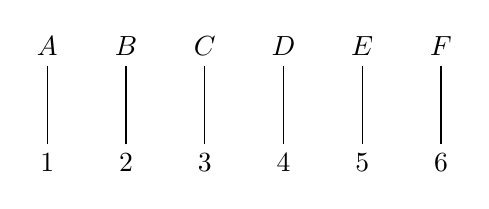
\begin{tikzpicture}

    \foreach \no/\a/\b in {
        0/$A$/1,
        1/$B$/2,
        2/$C$/3,
        3/$D$/4,
        4/$E$/5,
        5/$F$/6,
    }{
        \draw (\no,0) -- (\no,\height);
        \draw (\no,\height) node[above] {\a};
        \draw (\no,0) node[below] {\b};
    }

\end{tikzpicture}

\end{document}
